\documentclass[spanish,12pt,a4paper,titlepage]{report}
\usepackage[utf8]{inputenc}
\usepackage{graphicx}
\usepackage{subfig}
\usepackage{float}
\usepackage{wrapfig}
\usepackage{multirow}
\usepackage{caption}
\usepackage[spanish]{babel}
\usepackage[dvips]{hyperref}
\usepackage{amssymb}
\usepackage{listings}
\usepackage{epsfig}
\usepackage{amsmath}
\usepackage{array}
\usepackage[table]{xcolor}
\usepackage{multirow}
%\usepackage[Sonny]{fncychap}
\usepackage[Lenny]{fncychap}
%\usepackage[Glenn]{fncychap}
%\usepackage[Conny]{fncychap}
%\usepackage[Rejne]{fncychap}
%\usepackage[Bjarne]{fncychap}
%\usepackage[Bjornstrup]{fncychap}

%\usepackage{subfiles}
%\usepackage{framed}

\setlength{\topmargin}{-1.5cm}
\setlength{\textheight}{25cm}
\setlength{\oddsidemargin}{0.3cm} 
\setlength{\textwidth}{15cm}
\setlength{\columnsep}{0cm}

\begin{document}

\chapter{GPS - Test 2}
\label{chap-gps-test-2}

\section{Objetivos}
%\ref{} agregar refs
%TODO esta ref es trucha! cambiar por la posta!!
\label{chap-gps-test-1}

En el capítulo anterior se comenzó a analizar la performance del GPS. Se intentó reconstruir un polígono, y se analizó el error al estimar la posición de un punto fijo. En este capítulo se continúa dicho análisis, repitiendo el procedimiento, pero con un polígono más grande, y tiempo más largos para la estimación de la posición de un punto fijo.

\section{Materiales}

\begin{itemize}
\item GPS.
\item Laptop.
\item Trípode (de fotografía.
\item Cinta métrica, pintura y cuerda.
\end{itemize}

\newpage
\section{Procedimiento}
\label{sec:gps2-procedimiento}

En esta prueba se trata de obtener el error del GPS en el plano paralelo a la tierra, es decir, el error en latitud y longitud.

El experimento que se diseñó consiste en marcar un rectángulo sobre el suelo (pasto), utilizando 6 puntos, con la siguiente disposición:

\begin{quote}
\begin{quote}
\begin{quote}
\begin{verbatim}

      Árbol              
 Árbol               Árbol
           Gente_q_me_va_a_afanar
      Árbol
 -- < -- < -- < -- < -- < -- < -- <
    calle que sube de la rambla
 -- > -- > -- > -- > -- > -- > -- > 
 3                2                1
 x ---- ---- ---- x ---- ---- ---- x
 |                                 |
 |                                 |
 
 |                                 |
 |                                 |
 x ---- ---- ---- x ---- ---- ---- x
 6                5                4

     Estacionamiento de la fac

 Orientación del GPS:

                    led
                     ^
                     |
                     |
                    usb

\end{verbatim}
\end{quote}
\end{quote}
\end{quote}

A diferencia del experimento de la sección \ref{chap-gps-test-1}, aqui todas líneas punteadas son de 6m de largo, en lugar de 1m. Resulta en un rectángulo de 6m por 12m.

Los pasos a seguir son los siguientes:

\begin{enumerate}
\item Construir el rectángulo sobre un superficie plana.
  \begin{itemize}
  \item Se utilizó pintura para marcar los vértices del triángulo.
  \item Para trazar uno de los lados de 12 metros (puntos 1,2 y 3), se fijó una cuerda de 12 metros (con el punto medio marcado) a un punto, y se extendió (sin estirarla). El principio (\verb+1+) y el final (\verb+3+) de la cuerda son vértices del polígono, y el punto medio (\verb+2+) es otro de los puntos de interés.
  \item Para construir perpendículares se utilizó una cuerda de 6m, y otra de 8.5m\footnote{Pitágoras: $8.5 \approx \sqrt{6^2 + 6^2} = 8.4852...$}. Uno de los extremos de la cuerda de 6 metros se fijó al \verb+1+, y uno de los extremos de la cuerda de 8.5m se fijó a \verb+2+. El punto donde ambas se intersectan corresponde a \verb+4+. Un procedimiento similar se siguió para determinar la ubicación de \verb+5+ y \verb+6+.
  \end{itemize}
\item Medir, con un metro, las distancias entre todos los puntos.
\item Utilizar mínimos cuadrados para minimizar el error entre las distancias esperadas, y las experimentales. Esto puede llevar a trabajar con un polígono que \textbf{no} sea un rectángulo, pero el error será menor que el que resultaría de usar los valores teóricos.
\item Fijar la altura y la orientación del GPS, y tomar medidas en cada uno de los puntos \verb+[1,2,3,4,5,6]+.
\item Tomar un punto como origen, y comparar la figura que resulta de los datos provenientes del GPS con las medidas tomadas con el metro.
\end{enumerate}

En la figura \ref{fig:tripode_con_plomada.jpg} se observa el trípode que sostiene al GPS. El objetivo era tener el GPS a una altura fija, y separado del piso. Al nivel del piso los rebotes degradan seriamente la performance del GPS. La cuerda que marca el lado del polígono, junto con las patas del trípode, se utilizaron para fijar la orientación del GPS durante el experimento.

\begin{figure} [h!]
  \centering
  \subfloat[Trípode de fotografía, con el GPS atado en lugar de la cámara..]{\label{fig:tripode_con_plomada.jpg}
  		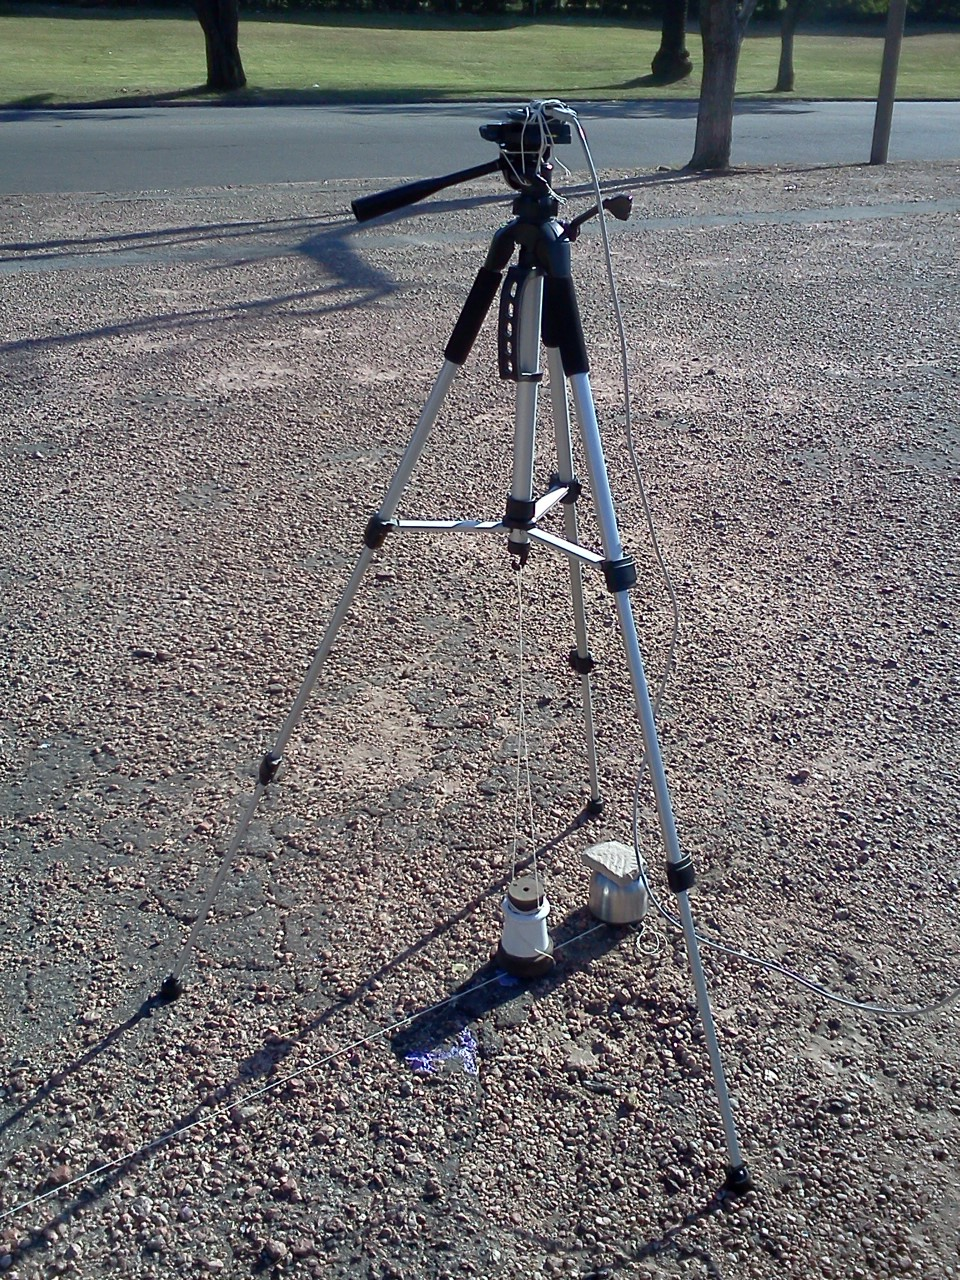
\includegraphics[width=0.45\textwidth]{./img/tripode_con_plomada.jpg}}
  \subfloat[GPS amarrado al trípode.]{\label{fig:vista_usb.jpg}
  		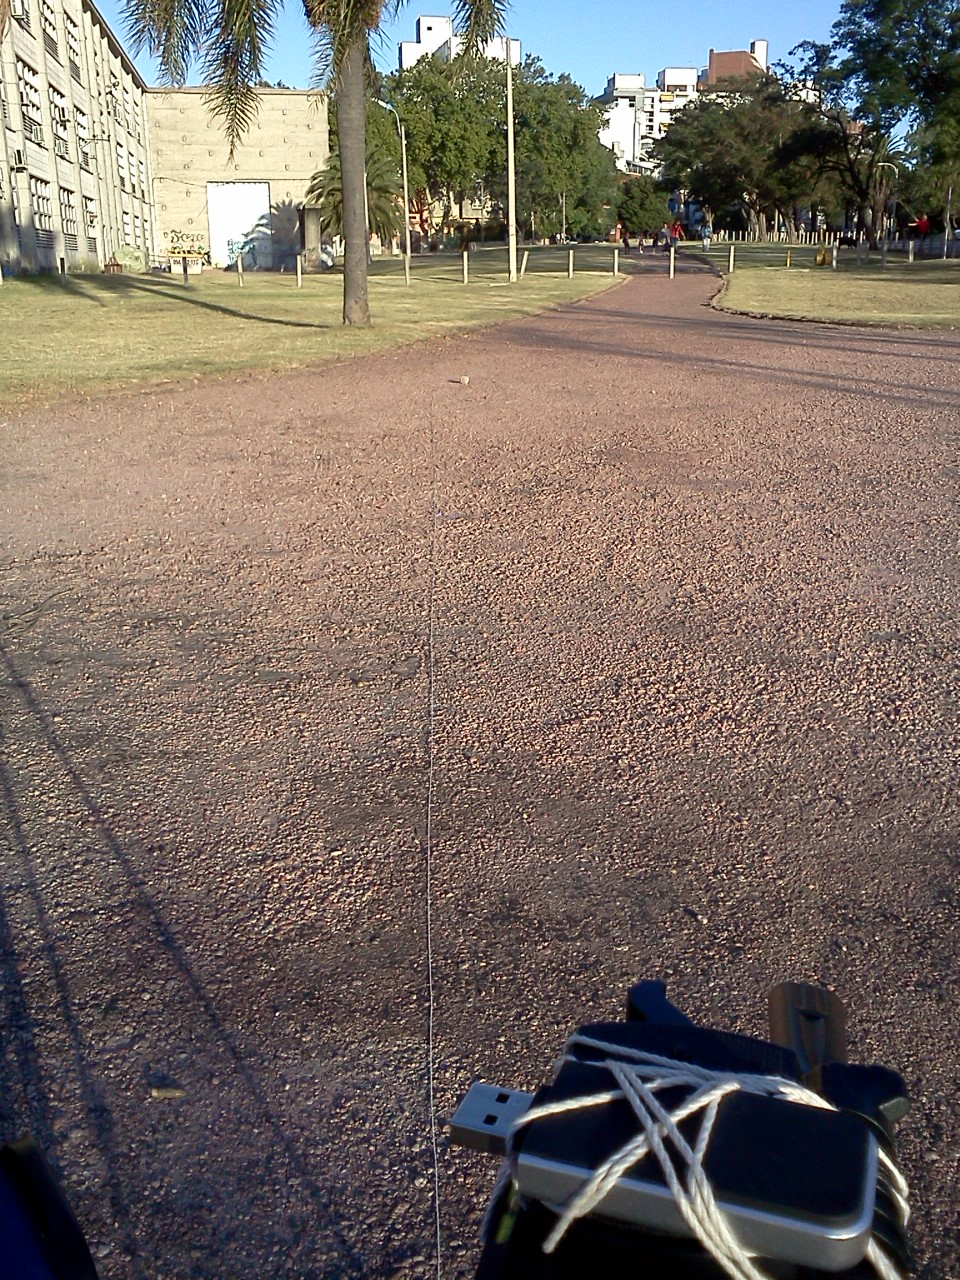
\includegraphics[width=0.45\textwidth]{./img/vista_usb.jpg}}
  \caption{Rebotes/Interferencia}
  \label{fig:rebotes}
\end{figure}

\newpage
\subsection{Verificación del polígono}
\label{sec:verificacion-del-poligono}

Una vez construído el polígono, es de interés medir todas las diagonales (con la cinta métrica) por dos motivos:
\begin{itemize}
\item Verificar que no se cometieron errores.
\item Hacer mínimos cuadrados con las medidas, de manera de obtener un polígono, que no tiene porqué ser (y en general no será) un rectángulo, sino algo similar a un rectángulo, más ajustado a la realidad.
\end{itemize}

Las medidas tomadas se resumen en la tabla \ref{tab:diagonales-poligono}, donde \verb+D12+ representa la medida de la recta que une el punto \verb+1+ con el punto \verb+2+, en cm.

\begin{table}[H]
\begin{center}
\begin{tabular}{|c|c|c|c|c|c|c|c|c|c|c|c|c|}
\hline
D12 & D14 & D15 & D16 & D23 & D24 & D25 & D26 & D34 & D35 & D36 & D45 & D56 \\
\hline
603 & 606 & 855 & 1345 & 603 & 853 & 608 & 853 & 1344 & 850 & 602 & 602 & 603 \\
\hline
\end{tabular}
\caption{Diagonales del polígono en cm. Lectura: $D42$ representa la longitud (en cm) de la recta que une el punto $4$ con el punto $2$.}
\label{tab:diagonales-poligono}
\end{center}
\end{table}

\newpage
\subsection{Punto fijo - 10 minutos}
\label{sec:gps2-punto-fijo-10-minutos}

Se tomaron datos durante 10 minutos ($\approx$ 600 muestras) en cada uno de los vértices del polígono, con el objetivo de observar la estabilidad de la información proveniente del GPS.

En la figura \ref{fig:10min_grid.png} se muestran los datos luego de restar el promedio, o sea que se muestra el error respecto al valor promedio.

\begin{figure}[h!]
  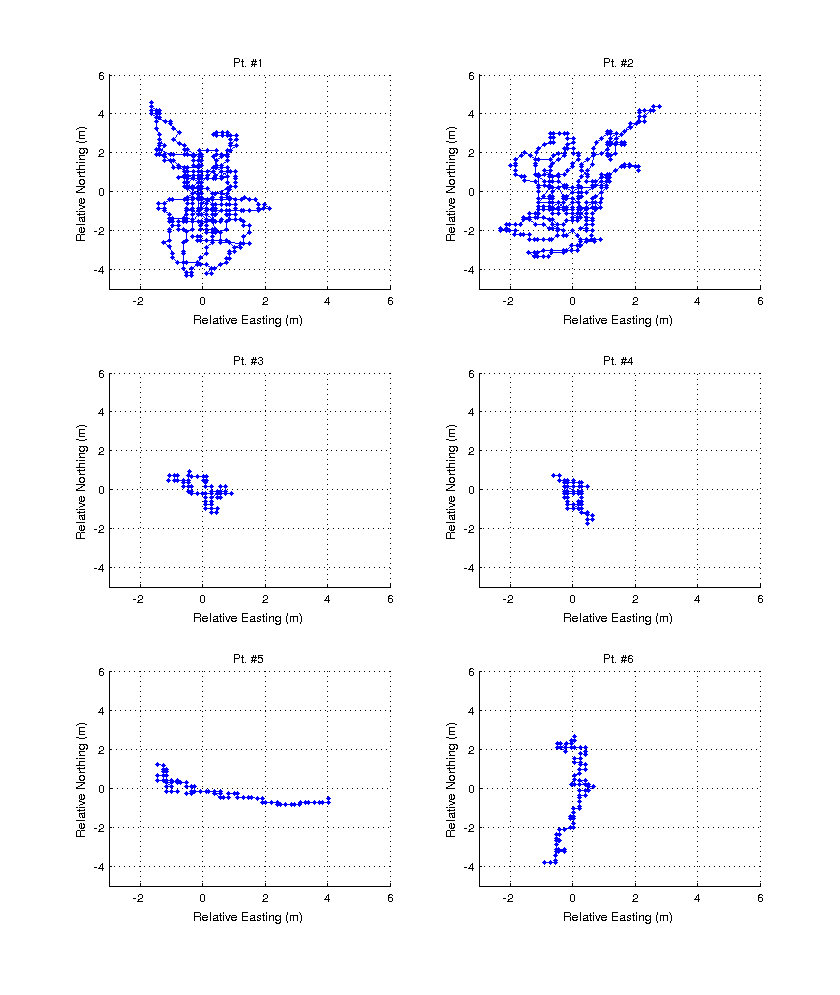
\includegraphics[width=1.1\textwidth]{./img/10min_grid.png}
  \caption{GPS quieto en cada punto del polígono, GPS orientado como en \ref{sec:gps2-procedimiento}.}
  \label{fig:10min_grid.png}
\end{figure}

\newpage
En la figura \ref{fig:10min_todos.png} se observan todas las gráficas de la figura \ref{fig:10min_grid.png}, pero superpuestas.

Si el GPS fuese perfecto, entonces todas las muestras coincidirían con el promedio, y estarían ubicadas en el punto \verb+[0,0]+. El círculo negro tiene 2.5m de radio, y fuera de él caen menos del 25\% de las muestras, para todos los puntos. Los datos para cada punto se observan en la tabla \ref{tab:fuera_del_circulo_10m}

\begin{table}[H]
\begin{center}
\begin{tabular}{|l|c|}
\hline
\textbf{Punto 1} & 25.4\% \\
\hline
\textbf{Punto 2} & 23.1\% \\
\hline
\textbf{Punto 3} & 0.0\% \\
\hline
\textbf{Punto 4} & 0.0\% \\
\hline
\textbf{Punto 5} & 11.5\% \\
\hline
\textbf{Punto 6} & 15.0\% \\
\hline
\end{tabular} 
\caption{Porcentaje de muestras \textbf{fuera} del círculo negro en la figura \ref{fig:10min_todos.png}.}
\label{tab:fuera_del_circulo_10m}
\end{center}
\end{table}

\begin{figure}[h!]
  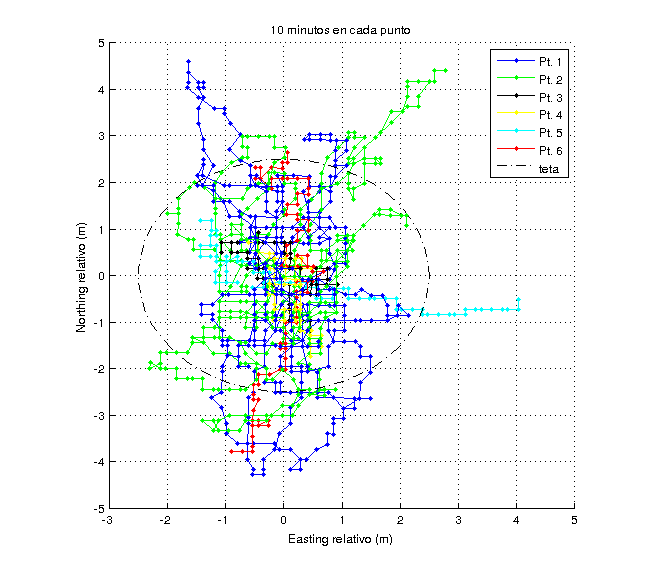
\includegraphics[width=1.1\textwidth]{./img/10min_todos.png}
  \caption{Error respecto al valor medio (Plots de \ref{fig:10min_grid.png} superpuestos).}
  \label{fig:10min_todos.png}
\end{figure}

El polígono resultante de dibujar las posiciones absolutas de los cada uno de los puntos se observa en la figura \ref{fig}

\subsubsection{Punto fijo - 10 minutos: Conclusiones}
\label{sec:gps2-punto-fijo-conclusiones}

%TODO

\textbf{HABRIA (VOY A) QUE HACER OTRA TIRADA PARA VER XQ CAMBIA TANTO LA COSA, A VER SI TIENE QUE VER CON 1 Y 2, O SI NA Q VER.}

\newpage
\subsection{Polígono}
\label{sec:gps2-poligono}

Se tomaron 2 minu

Intentando mejorar los resultados, se tomaron promedios en una ventana de 15 muestras, usando un filto \textit{moving average}. Esto también se observa en las figuras \ref{fig:polygon_1.png} y \ref{fig:polygon_2.png}.

% \begin{figure}[h!]
%   \begin{center}
%   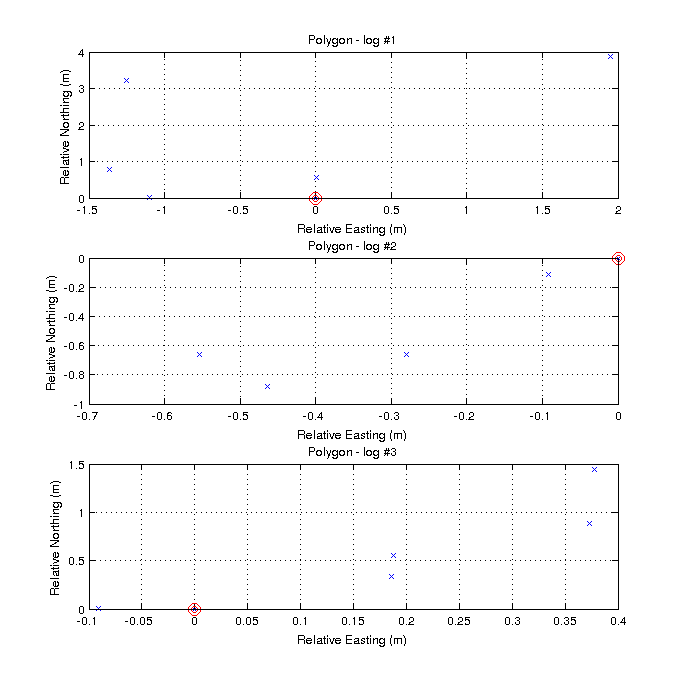
\includegraphics[width=1.1\textwidth]{./img/polygon_1.png}
%   \end{center}
%   \caption{Primeros 3 intentos de estimar el polígono.}
%   \label{fig:polygon_1.png}
% \end{figure}

% \newpage
% \begin{figure}[h!]
%   \begin{center}
%   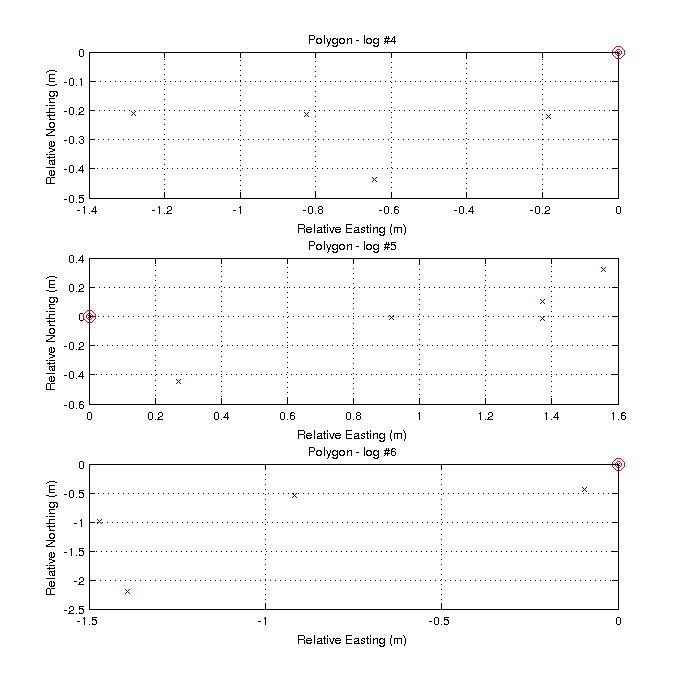
\includegraphics[width=1.1\textwidth]{./img/polygon_2.png}
%   \end{center}
%   \caption{Segundos 3 intentos de estimar el polígono.}
%   \label{fig:polygon_2.png}
% \end{figure}

\newpage
En la tabla \ref{tab:polygon-sat} se muestran la cantidad de satélites utilizados cuando se obtuvieron los datos de las figuras \ref{fig:polygon_1.png} y \ref{fig:polygon_2.png}.

\begin{table}[H]
\begin{center}
\begin{tabular}{|l||c|c|c|c|c|c|}
\hline
\textbf{Log 1} & 8 & 8 & 8 & 7 & 8 & 8 \\
\hline
\textbf{Log 2} & 9 & 9 & 9 & 9 & 9 & 9 \\
\hline
\textbf{Log 3} & 9 & 9 & 9 & 9 & 9 & 9 \\
\hline
\textbf{Log 4} & 10 & 10 & 10 & 10 & 10 & 10 \\
\hline
\textbf{Log 5} & 10 & 10 & 10 & 10 & 10 & 10 \\
\hline
\textbf{Log 6} & 10 & 10 & 10 & 10 & 10 & 10\\
\hline
\end{tabular} 
\caption{Satélites disponibles al tomar los datos de las figuras \ref{fig:polygon_1.png} y \ref{fig:polygon_2.png}.}
\label{tab:polygon-sat}
\end{center}
\end{table}

\subsubsection*{Errores}
\label{sec:errores}

Las especificaciones del GPS garantizan un error menor a 3m. La distancia de cada punto al punto 1 sirve para mostrar que el GPS cumple con las especificaciones. 

\begin{verbatim}
>> sqrt(easting.^2 + northing.^2)

ans =

  Columns 1 through 2

                         0                         0
         0.554512260087323         0.143700779969825
          4.33004706557553         0.143700779969825
          1.57529195895029         0.862204669928841
          3.46128113366155         0.997959241296461
          1.09657686103998           0.7196747757109

  Columns 3 through 4

                         0                         0
        0.0913813877153522         0.287401564952104
          0.37960034205882         0.287401564952104
         0.583854507635003         0.778438910449184
         0.959566360784181         0.851817377628425
          1.48734655792341          1.29842494542402

  Columns 5 through 6

                         0                         0
         0.521483162980721         0.452924086277894
          1.37072089636507         0.452924086277894
          1.58871200295859          1.06889681896435
         0.913813929586754          1.77030855041003
          1.37520004160367          2.60741605799409
\end{verbatim}

\newpage
Los datos crudos, antes de ser procesados, son los siguientes:

\begin{verbatim}
easting =
  Columns 1 through 2
          577829.024663918          577831.395779166
          577829.029379162          577831.303457993
          577830.976611558          577831.303457993
          577827.660593625          577830.841852163
          577827.772718459          577830.931344107
          577827.928126702           577831.11598643
  Columns 3 through 4
          577830.928514889          577830.394392373
          577830.837136806          577830.209750046
          577831.114100281          577830.209750046
           577831.11598643          577829.750973439
          577831.301571839          577829.570103359
          577831.306287223           577829.11321287
  Columns 5 through 6
            577828.8315342          577831.423128412
          577829.101896266          577831.327977979
          577830.202205538          577831.327977979
          577830.387790914          577830.504631801
          577829.745315091          577829.952590828
          577830.203148602          577830.033595277

northing =
  Columns 1 through 2
          6138921.43134999          6138920.85665408
           6138921.9858422          6138920.74653271
          6138925.29647715          6138920.74653271
          6138922.21929478          6138920.19592587
          6138924.65828346          6138919.97335191
          6138921.44067456          6138920.19359465
  Columns 3 through 4
          6138919.64065658          6138921.30879564
          6138919.64143365          6138921.08855289
          6138919.97179776          6138921.08855289
          6138920.19359465          6138920.87064132
          6138920.52473583          6138921.09399232
          6138921.07922804           6138921.0978776
  Columns 5 through 6
          6138920.21302122          6138924.07270891
          6138919.76709629          6138923.62989222
          6138920.20136535          6138923.62989222
          6138920.53250654          6138923.52598743
          6138920.20525066          6138923.08705604
          6138920.31226379          6138921.86639612
\end{verbatim}

\newpage
\begin{verbatim}
elevation =
  Columns 1 through 2
                        54                        54
                      50.4                        54
                      47.4                      53.9
                      44.5                      54.3
                      44.5                      54.4
                      47.9                      54.4
  Columns 3 through 4
                      54.5                        54
                      54.5                      54.2
                      54.5                      54.3
                      54.4                      54.5
                      54.2                      54.5
                      54.3                      53.9
  Columns 5 through 6
                      55.6                        56
                      56.4                      56.3
                      57.7                      56.3
                      57.8                      56.5
                      57.6                      56.6
                      57.5                      56.7
\end{verbatim}

 Cada columna corresponde a una serie. La columna 1 de easting va con la columna 1 de northing y la columna 1 de elevation, etc.

\subsection{Conclusión - Latitud-Longitud}
\label{sec:error-lat-lon-conclusion}

El GPS funciona como era de esperarse, con un error menor a 3m. Para estimar la posición del cuadricóptero con más precisión, va a ser necesario recurrir a sensores adicionales, o a algún tipo de manipulación de los datos del GPS.

No se calculó el error mediante mínimos cuadrados. Un análisis tan preciso no tiene sentido, ya que la magnitud del error es muy grande.

Este experimento se realizó libre de ruido. El cuadricóptero agregará vibraciones, interferencia electromagnética, y será mucho menos estable que el GPS aferrado a una escalera. El error en las medidas de este experimento fue, en general, significativamente menor a 3m, pero una vez montado en el cuadricóptero, es probable que el error en la información proveniente del GPS sea cercana a los 3m, por culpa de los factores mencionados.

%
%\begin{enumerate} 
%	\item Seleccionar 4 puntos distintos y asegurarse que estén a la misma altura. En lo posible formando un rectángulo siguiendo las direcciones de latitud y longitud, según lo indique la brújula.
%	\item Tomar las medidas con un metro lo más cuidadosamente posible entre los 4 vértices, y los ángulos que forman las parejas de caras consecutivas.
%	\item Obtener el dato del GPS de los 4 vértices.
%	\item Obtener la diferencia entre medidas
%	\item Convertir datos a unidades del sistema métrico.
%	\item Reproducir el paralelepípedo en un esquema según los datos obtenidos del GPS.
%	\item Contrastar medidas y ángulos reales con los obtenidos del GPS.
%\end{enumerate} 
%

\newpage
\section{Error en altura}
\label{sec:error-en-altura}

Para determinar el error la información sobre la altura que provee el GPS, se diseñó un experimento, que consiste en tomar medidas en una perpendicular a la esfera terrestre, a 4 alturas diferentes: 0m, 1m, 2m y 3m respecto al suelo.

En la primera etapa del experimento, se mantuvo el GPS quieto en cada uno de los niveles, y se tomaron muestras durante aproximadamente 60 segundos. El objetivo de esta etapa era verificar si era viable el experimento.

\subsection{Punto fijo}
\label{sec:altura-punto-fijo}

Para este experimento se colocó una escalera en el medio del estacionamiento de atrás de la Facultad de Ingeniería, se ató un piolín con marcas cada 1 metro, y una plomada en la punta para mantenerlo tenso y vertical.

% \begin{figure}[h!]
%   \begin{center}
%   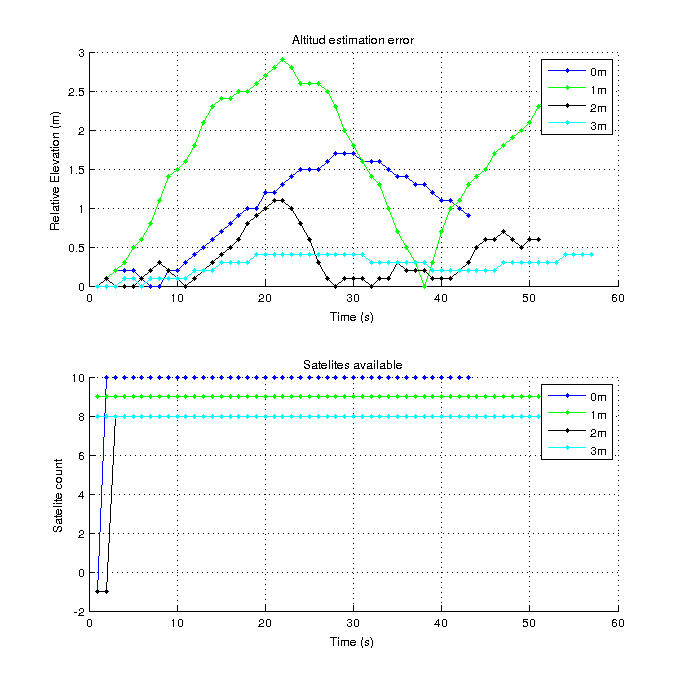
\includegraphics[width=.7\textwidth]{./img/altura_punto_fijo_fing.png}
%   \end{center}
%   \caption{Variación de la altura determinada por el GPS a distintas alturas.}
%   \label{fig:altura_punto_fijo_fing.png}
% \end{figure}

En la figura \ref{fig:altura_punto_fijo_fing.png} se observan los resultados del experimento. Es de esperarse que el error sea mayor al estar apoyado sobre el suelo, ya que los rebotes pueden deteriorar el sistema. El error a 1m de altura es mayor al que se obtuvo con el GPS en el suelo, una posible explicación para esto sería que el GPS estaba muy cerca de la escalera metálica, lo cual podría introducir una cantidad significativa de rebotes.

Los resultados de este experimento llevan a pensar que el GPS da información estable si y solo si se encuentra a al menos 2m del suelo. No se cuenta con suficiente información como para afirmar esto con certeza, por lo que se optó por tomar más datos, teniendo especial cuidado con el tema de los rebotes.

\subsection{Punto fijo - Estabilidad y rebotes}
\label{sec:altura-punto-fijo-estabilidad}

Para analizar el efecto de los rebotes sobre la estabilidad de la información proveniente del GPS, se tomaron varias series de datos con el GPS quieto, sobre el marco de una ventana, y luego asomado 1 metro hacia afuera (y arriba) de la ventana, donde el efecto de los rebotes debería ser menor.

En la figura \ref{fig:gps_gabi3.jpg} se observa la configuración del GPS al tomar los datos apoyado sobre el marco de la ventana, y en la figura \ref{fig:gps_gabi1.jpg} se observa el atril utilizado para alejar al GPS de la superficie.

% \begin{figure}[h!]
%   \begin{center}
% \subfloat[GPS expuesto a rebotes sobre la superficie en la que se apoya.]{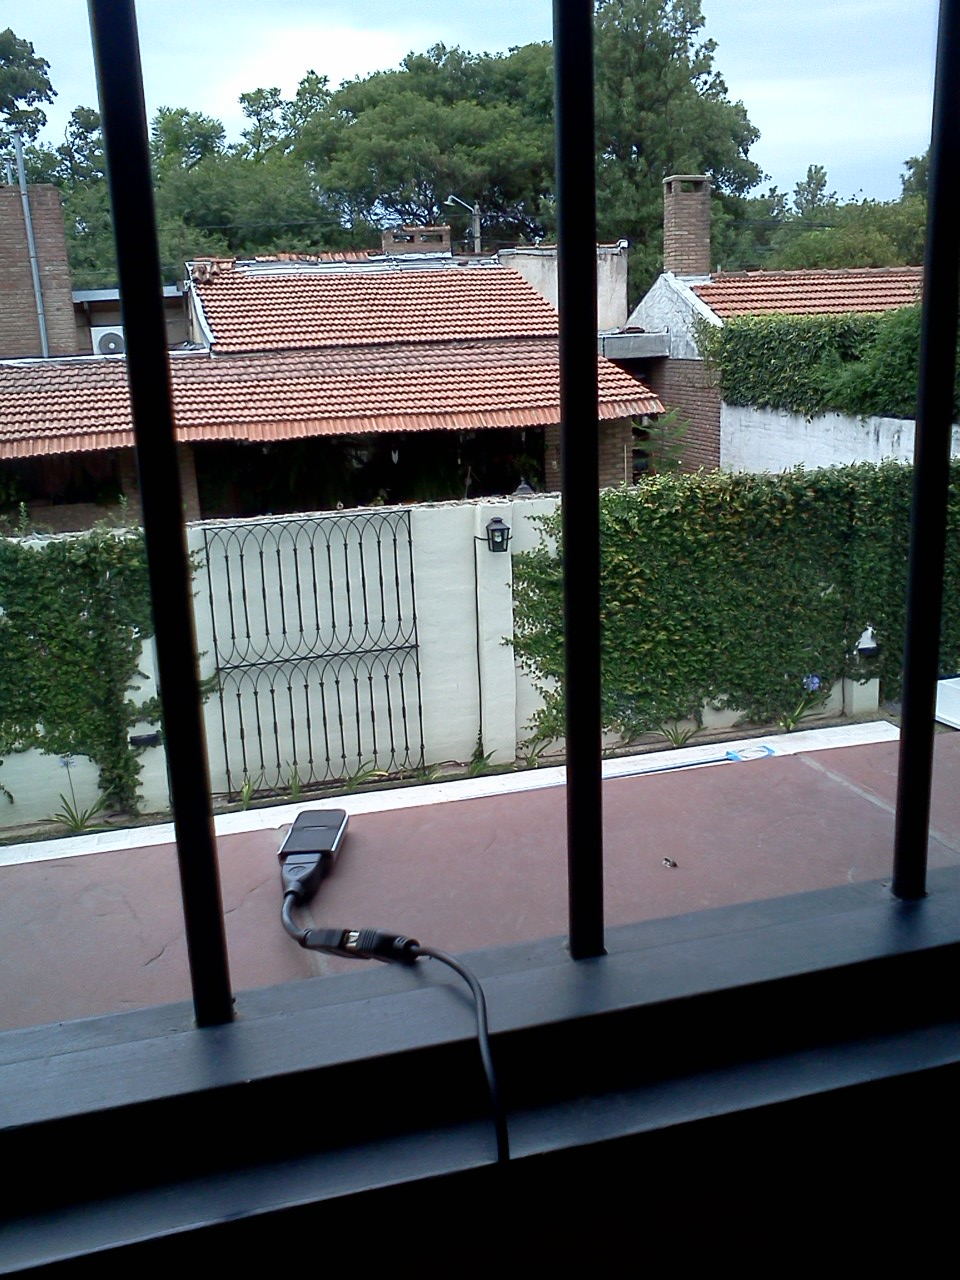
\includegraphics[width=.3\textwidth]{./img/gps_gabi3.jpg}\label{fig:gps_gabi1.jpg}}
% \hspace{50pt}
% \subfloat[GPS alejado de superficies.]{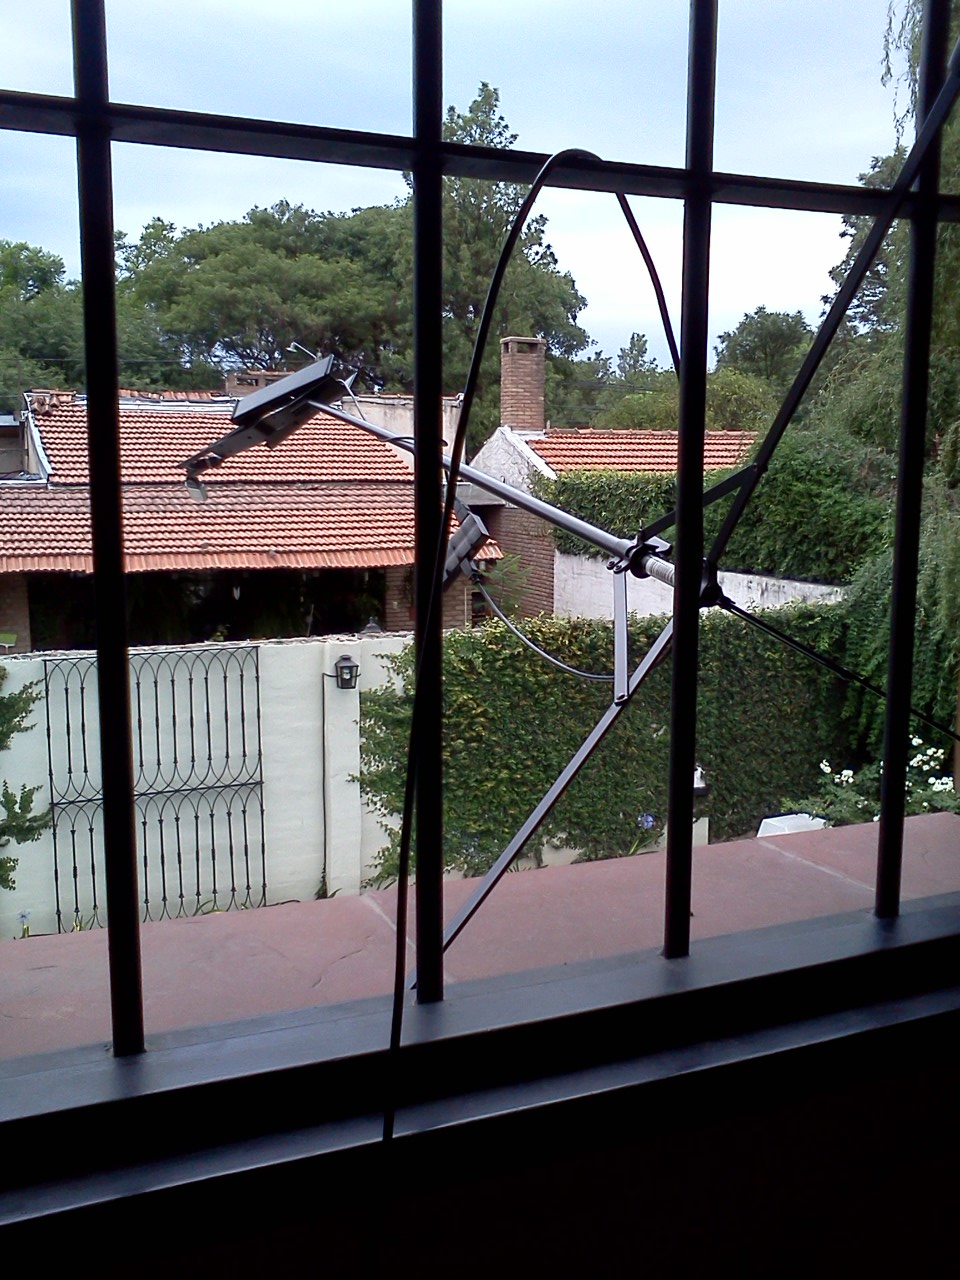
\includegraphics[width=.3\textwidth]{./img/gps_gabi1.jpg}\label{fig:gps_gabi3.jpg}}
%   \end{center}
% \end{figure}

Los resultados del experimento apoyado sobre el marco y asomado con el atril se observan en las figuras \ref{fig:gps_ventana.png} y \ref{fig:gps_atril.png} respectivamente.

% \begin{figure}[h!]
%   \begin{center}
%   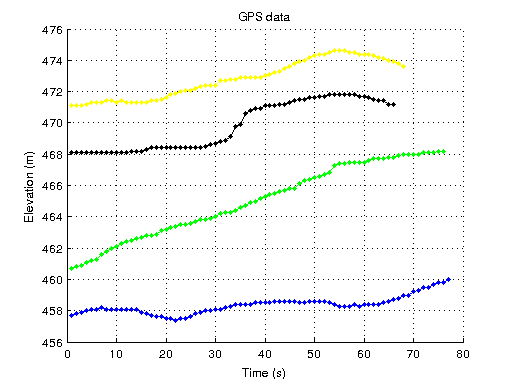
\includegraphics[width=.75\textwidth]{./img/gps_ventana.png}
%   \caption{GPS apoyado sobre superficie.}
%   \label{fig:gps_ventana.png}
% \end{center}
% \end{figure}

% \newpage
% \begin{figure}[h!]
% \begin{center}
%   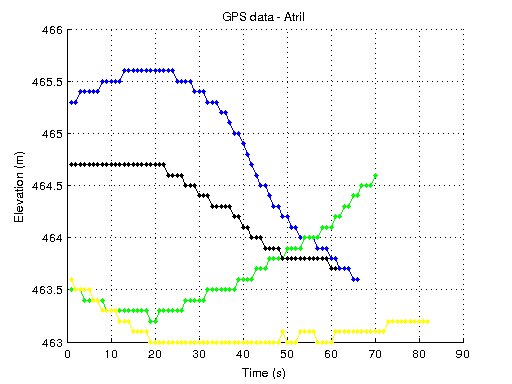
\includegraphics[width=.75\textwidth]{./img/gps_atril.png}
%   \caption{GPS alejado de superficies.}
%   \label{fig:gps_atril.png}
% \end{center}
% \end{figure}

\subsection{Conclusión - Altura}
\label{sec:error-en-altura-conclusion}

Los resultados concuerdan con lo esperado, la inestabilidad en la lectura del GPS disminuye al reducir las fuentes de rebotes.

Las lecturas del GPS no tiene suficiente precisión como para ser utilizadas de manera exclusiva para determinar la altura del cuadricóptero. En los mejores casos hay un error de $0.5-1$m, y en los peores casos hay errores de hasta 15m. Con una buena geometría y a varios metros del piso, el error es tolerable, pero no sirve para programar el aterrizaje/despegue, ni el vuelo a baja altura.

Aún no se ha determinado si la mayor causa del deterioro de la performance del GPS fueron los rebotes y/o la mala geometría. La mala geometría resulta de tener solamente la mitad del cielo visible, ya que la pared de la casa bloquea el resto. Al asomar el GPS hacia afuera, se lo aleja de los rebotes, y también se incrementa la cantidad de cielo visible, por lo que es difícil separar cual de los cambios es el responsable de los cambios en los resultados.

Se concluye que es necesario utilizar otra fuente de información, como por ejemplo un sensor de presión, para estimar la altura del cuadricóptero.

%\newpage

%\section{GPS con corrección diferencial}
%\label{sec:gps-diff}
%
%Para evaluar la performance del GPS en espacios más grandes, se relevó un polígono, tomando datos con el GPS a evaluar, junto con otro GPS que cuenta con correción diferencial, y es de mejor calidad.
%
%En la figura \ref se observa el camino recorrido, y los puntos de interés.
%
%\section{Parte III: Consistencia}
%
%Esta prueba se basa en la repetitividad de una misma prueba para analizar las diferencias entre los datos obtenidos por GPS en diferentes ocasiones.\\
%
%Se tomarán las medidas de los 4 puntos seleccionados en la parte anterior un total de 10 veces cada punto. Se analizarán los resultados obtenidos para caracterizar la consistencia del dispositivo GPS. Graficar las medidas obtenidas en latitud, longitud y altura para cada punto por separado. Hallar el error máximo de las medidas en un mismo punto.

%\section{Desarrollo}
%\subsection{Parte I: Error absoluto}
%
%\begin{table}[H]
%\begin{center}
%\begin{tabular}{|p{40pt}|p{110pt}|p{110pt}|p{110pt}|} 
%\hline
%  \cellcolor[gray]{0.8} \textbf{Medida} 
%& \cellcolor[gray]{0.8} \textbf{Posición 1} 
%& \cellcolor[gray]{0.8} \textbf{Posición 2} 
%& \cellcolor[gray]{0.8} \textbf{Posición 3} \\ \hline \hline
%\multicolumn{1}{|p{40pt}|}{\cellcolor[gray]{0.8}\textbf{1}} & \hspace{50pt}/ & \hspace{50pt}/ & \hspace{50pt}/ \\ \hline 
%\multicolumn{1}{|p{40pt}|}{\cellcolor[gray]{0.8}\textbf{2}} & \hspace{50pt}/& \hspace{50pt}/& \hspace{50pt}/ \\ \hline 
%\multicolumn{1}{|p{40pt}|}{\cellcolor[gray]{0.8}\textbf{3}} & \hspace{50pt}/& \hspace{50pt}/& \hspace{50pt}/ \\ \hline 
%\end{tabular} 
%\caption{Medidas GPS}
%\label{tab:I-medidas}
%\end{center}
%\end{table}
%
%\newpage
%\subsection{Parte II: Error relativo}
%
%\begin{table}[H]
%\begin{center}
%\begin{tabular}{|p{100pt}|p{100pt}|p{100pt}|p{100pt}|} \hline
%\cellcolor[gray]{0.8} \textbf{Punto 1} & \cellcolor[gray]{0.8} \textbf{Punto 2} & \cellcolor[gray]{0.8} \textbf{Punto 3} & \cellcolor[gray]{0.8} \textbf{Punto 4} \\ \hline \hline
%\hspace{50pt}/ & \hspace{50pt}/ & \hspace{50pt}/ & \hspace{50pt}/ \\ \hline 
%\end{tabular} 
%\caption{Medidas GPS}
%\label{tab:I-medidas}
%\end{center}
%\end{table}
%
%\newpage
%\subsection{Parte III: Consistencia}
%
%\begin{table}[H]
%\begin{center}
%\begin{tabular}{|p{40pt}|p{80pt}|p{80pt}|p{80pt}|p{80pt}|} \hline
%  \cellcolor[gray]{0.8} \textbf{Medida} 
%& \cellcolor[gray]{0.8} \textbf{Punto 1} 
%& \cellcolor[gray]{0.8} \textbf{Punto 2} 
%& \cellcolor[gray]{0.8} \textbf{Punto 3} 
%& \cellcolor[gray]{0.8} \textbf{Punto 4} \\ \hline \hline
%\multicolumn{1}{|p{40pt}|}{\cellcolor[gray]{0.8}\textbf{1}} & \hspace*{40pt}/& \hspace*{40pt}/& \hspace*{40pt}/& \hspace*{40pt}/\\ \hline 
%\multicolumn{1}{|p{40pt}|}{\cellcolor[gray]{0.8}\textbf{2}} & \hspace*{40pt}/& \hspace*{40pt}/& \hspace*{40pt}/& \hspace*{40pt}/\\ \hline 
%\multicolumn{1}{|p{40pt}|}{\cellcolor[gray]{0.8}\textbf{3}} & \hspace*{40pt}/& \hspace*{40pt}/& \hspace*{40pt}/& \hspace*{40pt}/\\ \hline
%\multicolumn{1}{|p{40pt}|}{\cellcolor[gray]{0.8}\textbf{4}} & \hspace*{40pt}/& \hspace*{40pt}/& \hspace*{40pt}/& \hspace*{40pt}/\\ \hline
%\multicolumn{1}{|p{40pt}|}{\cellcolor[gray]{0.8}\textbf{5}} & \hspace*{40pt}/& \hspace*{40pt}/& \hspace*{40pt}/& \hspace*{40pt}/\\ \hline
%\multicolumn{1}{|p{40pt}|}{\cellcolor[gray]{0.8}\textbf{6}} & \hspace*{40pt}/& \hspace*{40pt}/& \hspace*{40pt}/& \hspace*{40pt}/\\ \hline
%\multicolumn{1}{|p{40pt}|}{\cellcolor[gray]{0.8}\textbf{7}} & \hspace*{40pt}/& \hspace*{40pt}/& \hspace*{40pt}/& \hspace*{40pt}/\\ \hline
%\multicolumn{1}{|p{40pt}|}{\cellcolor[gray]{0.8}\textbf{8}} & \hspace*{40pt}/& \hspace*{40pt}/& \hspace*{40pt}/& \hspace*{40pt}/\\ \hline
%\multicolumn{1}{|p{40pt}|}{\cellcolor[gray]{0.8}\textbf{9}} & \hspace*{40pt}/& \hspace*{40pt}/& \hspace*{40pt}/& \hspace*{40pt}/\\ \hline
%\multicolumn{1}{|p{40pt}|}{\cellcolor[gray]{0.8}\textbf{10}} & \hspace*{40pt}/& \hspace*{40pt}/& \hspace*{40pt}/& \hspace*{40pt}/\\ \hline
%\end{tabular} 
%\caption{Toma de medidas}
%\label{tab:I-medidas}
%\end{center}
%\end{table}

\newpage
\section{Conclusión}
\label{sec:conclusion}

La performance del GPS cumple con lo especificado, en un contexto adecuado (buena geometría y buena visibilidad) da errores menores a 3m. Esto implica que el GPS no se puede utilizar para determinar la posición del cuadricóptero con una precisión razonable. Es de interés tener suficiente precisión como para poder maniobrar el cuadricóptero, y por lo tanto la posición se tiene que poder estimar con un error menor a 10cm.

La posición de la antena no parece afectar mucho los resultados, esto puede deberse a la geometría de la misma, es probable que tenga una cierta simetría que hace que la orientación del GPS no afecte la lecturas.

El GPS se utilizará como medio de corrección del drift que resulta de utilizar sensores que miden diferencias (acelerómetros, gyróscopos, etc), y estos otros sensores se usarán para obtener la precisión necesaria para maniobrar el cuadricóptero.

En cuanto a la estimación de la altura, no alcanza con el GPS, acelerómetros y gyróscopos, se requiere de un sonar, un sensor de presión, etc.

\end{document}